         \chapter{Electrostatics}\fancyfoot[LO,RE]{Physics: Electricity and Magnetism}
    \label{464e844ca5615087ea89d9d95dd9a43a}
         \section{Introduction and key concepts}
    \nopagebreak
%            \label{m38780} $ \hspace{-5pt}\begin{array}{cccccccccccc}   
\includegraphics[width=0.75cm]{col11305.imgs/summary_fullmarks.png} &   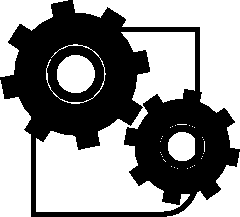
\includegraphics[width=0.75cm]{col11305.imgs/summary_simulation.png} &   \end{array} $ \hspace{2 pt}\raisebox{-5 pt}{} {(section shortcode: P10071 )} \par 
    \label{m38780*cid2}
       
      \label{m38780*id200254}Electrostatics is the study of electric charge which is static (not moving). In this chapter we will look at some of the basic principles of electrostatics as well as the principle of conservation of charge. \par 
    \label{m38780*cid3}
            \section{Two kinds of charge}
            \nopagebreak
      \label{m38780*id200267}All objects surrounding us (including people!) contain large amounts of electric charge. There
are two types of electric charge: \textbf{positive} charge and \textbf{negative} charge.
If the same amounts of negative and positive charge are found in an object, there
is \textsl{no net charge} and the object is charge \textbf{neutral}. If there is more of one type of charge than the other on the object then the object is said to be \textbf{electrically charged}. The picture below shows
what the distribution of charges might look like for a neutral, positively charged and
negatively charged object.\par 
      \label{m38780*id200640}
	\begin{figure}[H] % horizontal\label{m38780*id200643}
    \begin{center}
    \begin{pspicture}(0,-2.3017187)(13.100625,2.3017187)
\pscircle[linewidth=0.04,dimen=outer](1.6696875,-0.48828125){0.92}
\pscircle[linewidth=0.04,dimen=outer](6.2496877,-0.48828125){0.92}
\pscircle[linewidth=0.04,dimen=outer](10.789687,-0.46828124){0.92}
\rput(1.364375,0.10171875){+}
\rput(2.124375,-0.09828125){+}
\rput(2.184375,-0.87828124){+}
\rput(1.504375,-0.49828124){+}
\rput(1.364375,-1.1182812){+}
\rput(1.004375,-0.31828126){+}
\rput(1.1751562,-0.17828125){-}
\rput(1.5751562,0.04171875){-}
\rput(2.2551563,-0.19828124){-}
\rput(1.7351563,-0.45828125){-}
\rput(1.9951563,-0.97828126){-}
\rput(1.1751562,-0.91828126){-}
\rput(5.964375,0.08171875){+}
\rput(6.884375,-0.45828125){+}
\rput(5.624375,-0.35828125){+}
\rput(6.064375,-1.1782813){+}
\rput(6.404375,-0.35828125){+}
\rput(6.584375,-0.8382813){+}
\rput(5.784375,-0.8382813){+}
\rput(6.384375,0.00171875){+}
\rput(5.755156,0.00171875){-}
\rput(5.8351564,-0.41828126){-}
\rput(5.715156,-0.97828126){-}
\rput(6.215156,-1.0582813){-}
\rput(6.8951564,-0.61828125){-}
\rput(6.615156,0.04171875){-}
\rput(10.7951565,0.26171875){-}
\rput(11.084375,0.12171875){+}
\rput(11.384375,-0.43828124){+}
\rput(10.944375,-0.25828126){+}
\rput(10.784375,-1.1382812){+}
\rput(10.264375,-0.8382813){+}
\rput(10.364375,-0.21828125){+}
\rput(10.895156,-0.39828125){-}
\rput(11.395156,-0.6982812){-}
\rput(11.075156,-1.1182812){-}
\rput(10.395156,-0.9582813){-}
\rput(10.115156,-0.21828125){-}
\rput(10.595157,-0.59828126){-}
\rput(10.955156,-0.79828125){-}
\rput(10.475156,0.14171875){-}
\rput(1.019375,2.1217186){There are:}
\rput(1.7278125,1.4117187){\small 6 positive charges and}
\rput(1.4625,1.0517187){\small 6 negative charges}
\rput(1.66125,0.63171875){\small 6 + (-6) = 0}
\rput(1.6478125,-1.6882813){\small There is zero net charge:}
\rput(1.6682812,-2.0882812){\small The object is neutral}
\rput(6.284844,1.4117187){\small 8 positive charges and}
\rput(6.0225,1.0517187){\small 6 negative charges}
\rput(6.257344,0.63171875){\small 8 + (-6) = 2}
\rput(6.2725,-1.6882813){\small The net charge is +2}
\rput(6.33,-2.0882812){\small The object is positively charged}
\rput(10.787812,1.4117187){\small 6 positive charges and}
\rput(10.523125,1.0517187){\small 9 negative charges}
\rput(10.813281,0.63171875){\small 6 + (-9) = -3}
\rput(10.745469,-1.6882813){\small The net charge is -3}
\rput(10.87,-2.0882812){\small The object is negatively charged}
\end{pspicture}
\end{center}
 \end{figure}       
      \par \label{m38780*eip-429} Positive charge is carried by the protons in material and negative charge by electrons. The overall charge of an object is usually do to changes in the number of electrons.
      To make an object: 
      \begin{itemize}
       \item 	\textbf{Positively charged}: electrons are removed making the object electron \textbf{deficient}. 
	\item \textbf{Negatively charged}: electrons are added giving the object an \textbf{excess} of electrons.
      \end{itemize}
    So in practice what happens is that the number of positive charges (protons) remains the same and the number of electrons changes:
	\begin{figure}[H] % horizontal\label{m38780*id200643}
    \begin{center}
    \begin{pspicture}(0,-2.3017187)(13.100625,2.3017187)
\pscircle[linewidth=0.04,dimen=outer](1.6696875,-0.48828125){0.92}
\pscircle[linewidth=0.04,dimen=outer](6.2496877,-0.48828125){0.92}
\pscircle[linewidth=0.04,dimen=outer](10.789687,-0.46828124){0.92}
\rput(1.364375,0.10171875){+}
\rput(2.124375,-0.09828125){+}
\rput(2.184375,-0.87828124){+}
\rput(1.504375,-0.49828124){+}
\rput(1.364375,-1.1182812){+}
\rput(1.004375,-0.31828126){+}
\rput(1.1751562,-0.17828125){-}
\rput(1.5751562,0.04171875){-}
\rput(2.2551563,-0.19828124){-}
\rput(1.7351563,-0.45828125){-}
\rput(1.9951563,-0.97828126){-}
\rput(1.1751562,-0.91828126){-}
\rput(5.964375,0.08171875){+}
\rput(6.884375,-0.45828125){+}
\rput(5.624375,-0.35828125){+}
\rput(6.064375,-1.1782813){+}
\rput(6.404375,-0.35828125){+}
\rput(6.584375,-0.8382813){+}
% \rput(5.784375,-0.8382813){+}
% \rput(6.384375,0.00171875){+}
% \rput(5.755156,0.00171875){-}
% \rput(5.8351564,-0.41828126){-}
\rput(5.715156,-0.97828126){-}
\rput(6.215156,-1.0582813){-}
\rput(6.8951564,-0.61828125){-}
\rput(6.615156,0.04171875){-}
\rput(10.7951565,0.26171875){-}
\rput(11.084375,0.12171875){+}
\rput(11.384375,-0.43828124){+}
\rput(10.944375,-0.25828126){+}
\rput(10.784375,-1.1382812){+}
\rput(10.264375,-0.8382813){+}
\rput(10.364375,-0.21828125){+}
\rput(10.895156,-0.39828125){-}
\rput(11.395156,-0.6982812){-}
\rput(11.075156,-1.1182812){-}
\rput(10.395156,-0.9582813){-}
\rput(10.115156,-0.21828125){-}
\rput(10.595157,-0.59828126){-}
\rput(10.955156,-0.79828125){-}
\rput(10.475156,0.14171875){-}
\rput(1.019375,2.1217186){There are:}
\rput(1.7278125,1.4117187){\small \textbf{6} positive charges and}
\rput(1.4625,1.0517187){\small 6 negative charges}
\rput(1.66125,0.63171875){\small 6 + (-6) = 0}
\rput(1.6478125,-1.6882813){\small There is zero net charge:}
\rput(1.6682812,-2.0882812){\small The object is neutral}
\rput(6.284844,1.4117187){\small \textbf{6} positive charges and}
\rput(6.0225,1.0517187){\small 4 negative charges}
\rput(6.257344,0.63171875){\small 6 + (-4) = 2}
\rput(6.2725,-1.6882813){\small The net charge is +2}
\rput(6.33,-2.0882812){\small The object is positively charged}
\rput(10.787812,1.4117187){\small \textbf{6} positive charges and}
\rput(10.523125,1.0517187){\small 9 negative charges}
\rput(10.813281,0.63171875){\small 6 + (-9) = -3}
\rput(10.745469,-1.6882813){\small The net charge is -3}
\rput(10.87,-2.0882812){\small The object is negatively charged}
\end{pspicture}
\end{center}
 \end{figure}       



    \label{m38780*cid5}
            \subsection{Tribo-electric charging}
            \nopagebreak
            \label{m38780*id200729}Objects may become charged in many ways, including by contact with or being rubbed by other objects. This means that they can gain or lose negative charge. For example, charging happens
when you rub your feet against the carpet. When you
then touch something metallic or another person, you feel a shock as
the excess charge that you have collected is \textsl{discharged}.\par 
\Tip{Charge, like energy, cannot be created or destroyed. We say
that charge is \textbf{conserved}.}
\label{m38780*id200752}When you rub your feet
against the carpet, negative charge is transferred to you
from the carpet. The carpet will then become positively
charged by the \textsl{same amount}.\par 
      \label{m38780*id200762}Another example is to take two \textsl{neutral} objects such as a plastic ruler and a cotton cloth (handkerchief). To begin, the two objects are neutral (i.e. have the same amounts of positive and negative charge).\par 
      \label{m38780*id200774}
    \setcounter{subfigure}{0}
	\begin{figure}[H] % horizontal\label{m38780*id200777}
    \begin{center}
    \begin{pspicture}(0,-1.9746875)(14.900937,1.9746875)
\definecolor{color1034}{rgb}{0.6,0.6,0.6}
\psline[linewidth=0.04cm,linecolor=color1034](0.234375,0.67875)(0.234375,0.41875)
\psline[linewidth=0.04cm,linecolor=color1034](0.314375,0.69875)(0.314375,0.53875)
\psline[linewidth=0.04cm,linecolor=color1034](0.394375,0.69875)(0.394375,0.53875)
\psline[linewidth=0.04cm,linecolor=color1034](0.454375,0.69875)(0.454375,0.53875)
\psline[linewidth=0.04cm,linecolor=color1034](0.534375,0.69875)(0.534375,0.53875)
\psline[linewidth=0.04cm,linecolor=color1034](0.614375,0.67875)(0.614375,0.41875)
\psline[linewidth=0.04cm,linecolor=color1034](0.694375,0.69875)(0.694375,0.53875)
\psline[linewidth=0.04cm,linecolor=color1034](0.774375,0.69875)(0.774375,0.53875)
\psline[linewidth=0.04cm,linecolor=color1034](0.834375,0.69875)(0.834375,0.53875)
\psline[linewidth=0.04cm,linecolor=color1034](0.914375,0.69875)(0.914375,0.53875)
\psline[linewidth=0.04cm,linecolor=color1034](0.974375,0.67875)(0.974375,0.41875)
\psline[linewidth=0.04cm,linecolor=color1034](1.054375,0.69875)(1.054375,0.53875)
\psline[linewidth=0.04cm,linecolor=color1034](1.134375,0.69875)(1.134375,0.53875)
\psline[linewidth=0.04cm,linecolor=color1034](1.194375,0.69875)(1.194375,0.53875)
\psline[linewidth=0.04cm,linecolor=color1034](1.274375,0.69875)(1.274375,0.53875)
\psline[linewidth=0.04cm,linecolor=color1034](1.354375,0.67875)(1.354375,0.41875)
\psline[linewidth=0.04cm,linecolor=color1034](1.434375,0.69875)(1.434375,0.53875)
\psline[linewidth=0.04cm,linecolor=color1034](1.514375,0.69875)(1.514375,0.53875)
\psline[linewidth=0.04cm,linecolor=color1034](1.574375,0.69875)(1.574375,0.53875)
\psline[linewidth=0.04cm,linecolor=color1034](1.654375,0.69875)(1.654375,0.53875)
\psline[linewidth=0.04cm,linecolor=color1034](1.734375,0.67875)(1.734375,0.41875)
\psline[linewidth=0.04cm,linecolor=color1034](1.814375,0.69875)(1.814375,0.53875)
\psline[linewidth=0.04cm,linecolor=color1034](1.894375,0.69875)(1.894375,0.53875)
\psline[linewidth=0.04cm,linecolor=color1034](1.954375,0.69875)(1.954375,0.53875)
\psline[linewidth=0.04cm,linecolor=color1034](2.034375,0.69875)(2.034375,0.53875)
\psline[linewidth=0.04cm,linecolor=color1034](2.114375,0.67875)(2.114375,0.41875)
\psline[linewidth=0.04cm,linecolor=color1034](2.194375,0.69875)(2.194375,0.53875)
\psline[linewidth=0.04cm,linecolor=color1034](2.274375,0.69875)(2.274375,0.53875)
\psline[linewidth=0.04cm,linecolor=color1034](2.334375,0.69875)(2.334375,0.53875)
\psline[linewidth=0.04cm,linecolor=color1034](2.414375,0.69875)(2.414375,0.53875)
\psline[linewidth=0.04cm,linecolor=color1034](2.494375,0.67875)(2.494375,0.41875)
\psline[linewidth=0.04cm,linecolor=color1034](2.574375,0.69875)(2.574375,0.53875)
\psline[linewidth=0.04cm,linecolor=color1034](2.654375,0.69875)(2.654375,0.53875)
\psline[linewidth=0.04cm,linecolor=color1034](2.714375,0.69875)(2.714375,0.53875)
\psline[linewidth=0.04cm,linecolor=color1034](2.794375,0.69875)(2.794375,0.53875)
\psline[linewidth=0.04cm,linecolor=color1034](2.874375,0.67875)(2.874375,0.41875)
\psline[linewidth=0.04cm,linecolor=color1034](2.954375,0.69875)(2.954375,0.53875)
\psline[linewidth=0.04cm,linecolor=color1034](3.034375,0.69875)(3.034375,0.53875)
\psline[linewidth=0.04cm,linecolor=color1034](3.094375,0.69875)(3.094375,0.53875)
\psline[linewidth=0.04cm,linecolor=color1034](3.174375,0.69875)(3.174375,0.53875)
\psline[linewidth=0.04cm,linecolor=color1034](3.254375,0.67875)(3.254375,0.41875)
\psline[linewidth=0.04cm,linecolor=color1034](3.334375,0.69875)(3.334375,0.53875)
\psline[linewidth=0.04cm,linecolor=color1034](3.414375,0.69875)(3.414375,0.53875)
\psline[linewidth=0.04cm,linecolor=color1034](3.474375,0.69875)(3.474375,0.53875)
\psline[linewidth=0.04cm,linecolor=color1034](3.554375,0.69875)(3.554375,0.53875)
\psline[linewidth=0.04cm,linecolor=color1034](3.634375,0.67875)(3.634375,0.41875)
\psline[linewidth=0.04cm,linecolor=color1034](3.714375,0.69875)(3.714375,0.53875)
\psline[linewidth=0.04cm,linecolor=color1034](3.794375,0.69875)(3.794375,0.53875)
\psline[linewidth=0.04cm,linecolor=color1034](3.854375,0.69875)(3.854375,0.53875)
\psline[linewidth=0.04cm,linecolor=color1034](3.934375,0.69875)(3.934375,0.53875)
\psline[linewidth=0.04cm,linecolor=color1034](4.014375,0.67875)(4.014375,0.41875)
\psline[linewidth=0.04cm,linecolor=color1034](4.094375,0.69875)(4.094375,0.53875)
\psline[linewidth=0.04cm,linecolor=color1034](4.174375,0.69875)(4.174375,0.53875)
\psline[linewidth=0.04cm,linecolor=color1034](4.234375,0.69875)(4.234375,0.53875)
\psline[linewidth=0.04cm,linecolor=color1034](4.314375,0.69875)(4.314375,0.53875)
\psline[linewidth=0.04cm,linecolor=color1034](4.394375,0.67875)(4.394375,0.41875)
\psline[linewidth=0.04cm,linecolor=color1034](4.474375,0.69875)(4.474375,0.53875)
\psline[linewidth=0.04cm,linecolor=color1034](4.554375,0.69875)(4.554375,0.53875)
\psline[linewidth=0.04cm,linecolor=color1034](4.614375,0.69875)(4.614375,0.53875)
\psline[linewidth=0.04cm,linecolor=color1034](4.694375,0.69875)(4.694375,0.53875)
\psline[linewidth=0.04cm,linecolor=color1034](4.794375,0.69875)(4.794375,0.43875)
\psframe[linewidth=0.04,dimen=outer](5.234375,0.69875)(0.054375,-0.02125)
\rput(4.9290624,0.24875){+}
\rput(4.4090624,0.24875){+}
\rput(3.8690624,0.22875){+}
\rput(3.3290625,0.22875){+}
\rput(2.7090626,0.24875){+}
\rput(2.1890626,0.24875){+}
\rput(1.7090625,0.22875){+}
\rput(1.1490625,0.22875){+}
\rput(0.5090625,0.20875){+}
\rput(0.21984375,0.24875){-}
\rput(0.81984377,0.20875){-}
\rput(1.3998437,0.24875){-}
\rput(1.9198438,0.28875){-}
\rput(2.4198437,0.28875){-}
\rput(2.9598436,0.24875){-}
\rput(3.6198437,0.24875){-}
\rput(4.119844,0.28875){-}
\rput(4.639844,0.26875){-}
\psbezier[linewidth=0.04](6.042201,1.0521983)(5.814375,1.19875)(6.6262674,-0.91064626)(6.6262674,-0.53135264)(6.6262674,-0.152059)(8.434375,-1.02125)(8.401829,-0.5882467)(8.369282,-0.15524337)(7.636984,0.64375)(7.86481,0.8406855)(8.092636,1.037621)(6.270027,0.9056466)(6.042201,1.0521983)
\rput(6.6290627,0.62875){+}
\rput(7.4490623,0.30875){+}
\rput(6.6690626,-0.09125){+}
\rput(7.6490626,-0.37125){+}
\rput(7.3090625,0.76875){+}
\rput(6.4598436,0.48875){-}
\rput(6.8798437,0.08875){-}
\rput(7.9598436,-0.37125){-}
\rput(7.5398436,0.12875){-}
\rput(7.099844,0.66875){-}
\rput(2.4446876,-0.34125){\small The ruler has 9 positive charges and}
\rput(7.749375,-1.12125){\small The neutral cotton cloth has}
\rput(7.7117186,-1.44125){\small 5 positive charges and}
\rput(7.726406,-1.76125){\small 5 negative charges}
\rput(12.6725,0.91875){\small The total number of charges is:}
\rput(12.3175,0.49875){\small (9+5)=14 positive charges}
\rput(12.3375,0.11875){\small (9+5)=14 negative charges}
\rput(1.3078125,-0.68125){\small 9 negative charges}
\rput(1.2048438,1.79875){\small BEFORE rubbing:}
\end{pspicture}\end{center}
 \end{figure}       
      \par 
      \label{m38780*id200783}Now, if the cotton cloth is used to rub the ruler, negative charge
is transferred \textsl{from} the cloth \textsl{to} the ruler.
The ruler is now \textsl{negatively} charged (i.e. has an excess of electrons) and the cloth is \textsl{positively} charged (i.e. is electron deficient).
If you count up all the positive and negative charges at the beginning and the end, there are still the same amount. i.e. total charge has been \textsl{conserved}!\par 
      \label{m38780*id200814}
    \setcounter{subfigure}{0}
	\begin{figure}[H] % horizontal\label{m38780*id200819}
    \begin{center}
    \begin{pspicture}(0,-2.1746874)(15.098437,2.1746874)
\definecolor{color1034}{rgb}{0.6,0.6,0.6}
\psline[linewidth=0.04cm,linecolor=color1034](0.2371875,0.87875)(0.2371875,0.61875)
\psline[linewidth=0.04cm,linecolor=color1034](0.3171875,0.89875)(0.3171875,0.73875)
\psline[linewidth=0.04cm,linecolor=color1034](0.3971875,0.89875)(0.3971875,0.73875)
\psline[linewidth=0.04cm,linecolor=color1034](0.4571875,0.89875)(0.4571875,0.73875)
\psline[linewidth=0.04cm,linecolor=color1034](0.5371875,0.89875)(0.5371875,0.73875)
\psline[linewidth=0.04cm,linecolor=color1034](0.6171875,0.87875)(0.6171875,0.61875)
\psline[linewidth=0.04cm,linecolor=color1034](0.6971875,0.89875)(0.6971875,0.73875)
\psline[linewidth=0.04cm,linecolor=color1034](0.7771875,0.89875)(0.7771875,0.73875)
\psline[linewidth=0.04cm,linecolor=color1034](0.8371875,0.89875)(0.8371875,0.73875)
\psline[linewidth=0.04cm,linecolor=color1034](0.9171875,0.89875)(0.9171875,0.73875)
\psline[linewidth=0.04cm,linecolor=color1034](0.9771875,0.87875)(0.9771875,0.61875)
\psline[linewidth=0.04cm,linecolor=color1034](1.0571876,0.89875)(1.0571876,0.73875)
\psline[linewidth=0.04cm,linecolor=color1034](1.1371875,0.89875)(1.1371875,0.73875)
\psline[linewidth=0.04cm,linecolor=color1034](1.1971875,0.89875)(1.1971875,0.73875)
\psline[linewidth=0.04cm,linecolor=color1034](1.2771875,0.89875)(1.2771875,0.73875)
\psline[linewidth=0.04cm,linecolor=color1034](1.3571875,0.87875)(1.3571875,0.61875)
\psline[linewidth=0.04cm,linecolor=color1034](1.4371876,0.89875)(1.4371876,0.73875)
\psline[linewidth=0.04cm,linecolor=color1034](1.5171875,0.89875)(1.5171875,0.73875)
\psline[linewidth=0.04cm,linecolor=color1034](1.5771875,0.89875)(1.5771875,0.73875)
\psline[linewidth=0.04cm,linecolor=color1034](1.6571875,0.89875)(1.6571875,0.73875)
\psline[linewidth=0.04cm,linecolor=color1034](1.7371875,0.87875)(1.7371875,0.61875)
\psline[linewidth=0.04cm,linecolor=color1034](1.8171875,0.89875)(1.8171875,0.73875)
\psline[linewidth=0.04cm,linecolor=color1034](1.8971875,0.89875)(1.8971875,0.73875)
\psline[linewidth=0.04cm,linecolor=color1034](1.9571875,0.89875)(1.9571875,0.73875)
\psline[linewidth=0.04cm,linecolor=color1034](2.0371876,0.89875)(2.0371876,0.73875)
\psline[linewidth=0.04cm,linecolor=color1034](2.1171875,0.87875)(2.1171875,0.61875)
\psline[linewidth=0.04cm,linecolor=color1034](2.1971874,0.89875)(2.1971874,0.73875)
\psline[linewidth=0.04cm,linecolor=color1034](2.2771876,0.89875)(2.2771876,0.73875)
\psline[linewidth=0.04cm,linecolor=color1034](2.3371875,0.89875)(2.3371875,0.73875)
\psline[linewidth=0.04cm,linecolor=color1034](2.4171875,0.89875)(2.4171875,0.73875)
\psline[linewidth=0.04cm,linecolor=color1034](2.4971876,0.87875)(2.4971876,0.61875)
\psline[linewidth=0.04cm,linecolor=color1034](2.5771875,0.89875)(2.5771875,0.73875)
\psline[linewidth=0.04cm,linecolor=color1034](2.6571875,0.89875)(2.6571875,0.73875)
\psline[linewidth=0.04cm,linecolor=color1034](2.7171874,0.89875)(2.7171874,0.73875)
\psline[linewidth=0.04cm,linecolor=color1034](2.7971876,0.89875)(2.7971876,0.73875)
\psline[linewidth=0.04cm,linecolor=color1034](2.8771875,0.87875)(2.8771875,0.61875)
\psline[linewidth=0.04cm,linecolor=color1034](2.9571874,0.89875)(2.9571874,0.73875)
\psline[linewidth=0.04cm,linecolor=color1034](3.0371876,0.89875)(3.0371876,0.73875)
\psline[linewidth=0.04cm,linecolor=color1034](3.0971875,0.89875)(3.0971875,0.73875)
\psline[linewidth=0.04cm,linecolor=color1034](3.1771874,0.89875)(3.1771874,0.73875)
\psline[linewidth=0.04cm,linecolor=color1034](3.2571876,0.87875)(3.2571876,0.61875)
\psline[linewidth=0.04cm,linecolor=color1034](3.3371875,0.89875)(3.3371875,0.73875)
\psline[linewidth=0.04cm,linecolor=color1034](3.4171875,0.89875)(3.4171875,0.73875)
\psline[linewidth=0.04cm,linecolor=color1034](3.4771874,0.89875)(3.4771874,0.73875)
\psline[linewidth=0.04cm,linecolor=color1034](3.5571876,0.89875)(3.5571876,0.73875)
\psline[linewidth=0.04cm,linecolor=color1034](3.6371875,0.87875)(3.6371875,0.61875)
\psline[linewidth=0.04cm,linecolor=color1034](3.7171874,0.89875)(3.7171874,0.73875)
\psline[linewidth=0.04cm,linecolor=color1034](3.7971876,0.89875)(3.7971876,0.73875)
\psline[linewidth=0.04cm,linecolor=color1034](3.8571875,0.89875)(3.8571875,0.73875)
\psline[linewidth=0.04cm,linecolor=color1034](3.9371874,0.89875)(3.9371874,0.73875)
\psline[linewidth=0.04cm,linecolor=color1034](4.0171876,0.87875)(4.0171876,0.61875)
\psline[linewidth=0.04cm,linecolor=color1034](4.0971875,0.89875)(4.0971875,0.73875)
\psline[linewidth=0.04cm,linecolor=color1034](4.1771874,0.89875)(4.1771874,0.73875)
\psline[linewidth=0.04cm,linecolor=color1034](4.2371874,0.89875)(4.2371874,0.73875)
\psline[linewidth=0.04cm,linecolor=color1034](4.3171873,0.89875)(4.3171873,0.73875)
\psline[linewidth=0.04cm,linecolor=color1034](4.3971877,0.87875)(4.3971877,0.61875)
\psline[linewidth=0.04cm,linecolor=color1034](4.4771876,0.89875)(4.4771876,0.73875)
\psline[linewidth=0.04cm,linecolor=color1034](4.5571876,0.89875)(4.5571876,0.73875)
\psline[linewidth=0.04cm,linecolor=color1034](4.6171875,0.89875)(4.6171875,0.73875)
\psline[linewidth=0.04cm,linecolor=color1034](4.6971874,0.89875)(4.6971874,0.73875)
\psline[linewidth=0.04cm,linecolor=color1034](4.7971873,0.89875)(4.7971873,0.63875)
\psframe[linewidth=0.04,dimen=outer](5.2371874,0.89875)(0.0571875,0.17875)
\rput(4.931875,0.44875){+}
\rput(4.411875,0.44875){+}
\rput(3.871875,0.42875){+}
\rput(3.331875,0.42875){+}
\rput(2.711875,0.44875){+}
\rput(2.191875,0.44875){+}
\rput(1.711875,0.42875){+}
\rput(1.151875,0.42875){+}
\rput(0.511875,0.40875){+}
\rput(0.22265625,0.44875){-}
\rput(0.8226563,0.40875){-}
\rput(1.4026562,0.44875){-}
\rput(1.9226563,0.48875){-}
\rput(2.4226563,0.48875){-}
\rput(2.9626563,0.44875){-}
\rput(3.6226563,0.44875){-}
\rput(4.1226563,0.48875){-}
\rput(4.6426563,0.46875){-}
\psbezier[linewidth=0.04](6.0450134,1.2521983)(5.8171873,1.39875)(6.62908,-0.7106463)(6.62908,-0.33135265)(6.62908,0.047941)(8.437187,-0.82125)(8.404641,-0.3882467)(8.372094,0.04475663)(7.6397963,0.84375)(7.8676224,1.0406855)(8.0954485,1.237621)(6.2728395,1.1056466)(6.0450134,1.2521983)
\rput(6.631875,0.82875){+}
\rput(7.451875,0.50875){+}
\rput(6.671875,0.10875){+}
\rput(7.651875,-0.17125){+}
\rput(7.311875,0.96875){+}
\rput(4.9826565,0.72875){-}
\rput(5.0426564,0.34875){-}
\rput(7.962656,-0.17125){-}
\rput(7.5426564,0.32875){-}
\rput(4.6226563,0.62875){-}
\rput(2.4475,-0.14125){\small The ruler has 9 positive charges and}
\rput(7.4821873,-0.92125){\small The cotton cloth has}
\rput(7.614531,-1.24125){\small 5 positive charges and}
\rput(7.3940625,-1.58125){\small 2 negative charges.}
\rput(12.585313,1.11875){\small The total number of charges is:}
\rput(12.3203125,0.69875){\small (9+5)=14 positive charges}
\rput(12.430312,0.31875){\small (12+2)=14 negative charges}
\rput(1.3873438,-0.48125){\small 12 negative charges}
\rput(1.0790625,1.99875){\small AFTER rubbing:}
\rput(7.6434374,-1.96125){\small It is now positively charged.}
\rput(2.0234375,-0.84125){\small It is now negatively charged.}
\rput(12.391719,-0.28125){\small Charges have been transferred from the}
\rput(12.3515625,-0.64125){\small cloth to the ruler BUT total charge has}
\rput(10.865313,-0.98125){\small been conserved!}
\end{pspicture}\end{center}
 \end{figure}       
 \par 
\begin{minipage}{.4\textwidth}

      \label{m38780*id200825}Note that in this example the numbers are made up to be easy to calculate. In the real world only a tiny fraction of the charges would move from one object to the other, but the total charge would still be conserved.\par \Tip{This simulation will help you understand what happens when you rub an object against another object. \raisebox{-5 pt}{ 
\includegraphics[width=0.5cm]{col11305.imgs/summary_www.png}} {(Simulation: lbX)}}
The process of materials becoming charged when they come into contact with other materials is known as tribo-electric charging. Materials can be arranged in a tribo-electric series according to whether they are more positive or more negative. This tribo-electric series can allow us to determine whether one material is likely to become charged from another material. 

Positive materials are more likely to lose electrons and negative materials are more likely to gain. So when two materials are chosen and rubbed together the one that is more positive in the series will lose electrons and the one that is negative in the series will gain electrons.
 For example, amber is more negative than wool and so if a piece of wool is rubbed against a piece of amber then the amber will become negatively charged.\end{minipage}
\begin{minipage}{.6\textwidth}
\begin{center}
\begin{table}[H]
\centering
\begin{tabular}{|cc|}\hline
\textbf{Material}&\textbf{Tribo-electric series}\\\hline
Glass& Very positive\\\hline
Human hair&\\\hline
Nylon&\\\hline
Wool&\\\hline
Fur&\\\hline
Lead&\\\hline
Silk&\\\hline
Aluminum&\\\hline
Paper&\\\hline
Cotton&Neutral\\\hline
Steel &Neutral\\\hline
Wood&\\\hline
Amber&\\\hline
Hard rubber&\\\hline
Nickel, Copper&\\\hline
Gold, Platinum&\\\hline
Polyester&\\\hline
Polyurethane&\\\hline
Polypropylene&\\\hline
Silicon&\\\hline
Teflon& Very negative\\\hline
\end{tabular}
\caption{Tribo-electric series.}
\end{table}
\end{center}
\end{minipage}

\begin{wex}{Tribo-electric charging}
{If you have a cotton cloth and a silk cloth and you rub them together, which becomes negatively charged?}
{\westep{Analyse the information provided}
There are two materials provided and they will be rubbed together. This means we are dealing with the interaction between the materials. The question is related to the charge on the materials which we can assume were neutral to begin with. This means that we are dealing electrostatics and the interaction of materials leading to the materials becoming charged is tribo-electric charging.
\westep{Extract material properties}
Locate the materials in the tribo-electric series. The key thing is to know which is more positive and more negative in the series. Silk falls above cotton in our table making it more positive in the series.
\westep{Apply principles}
We know that when two materials are rubbed the more negative one in the series gains electrons and the more positive one loses electrons. This means that silk will lose electrons and cotton will gain electrons.
\par
A material becomes negatively charged when it has an excess of electrons, thus the cotton, which gains electrons, becomes negatively charged.}\end{wex}

    \label{m38780*cid6}
            \subsection{Force between charges}
            \nopagebreak
            \label{m38780*id200840}The force exerted by non-moving (static) charges on each other is called the \textbf{electrostatic force.} The electrostatic force between:\par 
      \label{m38780*id200849}\begin{itemize}[noitemsep]
            \label{m38780*uid1}\item \textbf{like} charges is \textbf{repulsive}\label{m38780*uid2}\item \textbf{opposite} (unlike) charges is \textbf{attractive}.
\end{itemize}
      \label{m38780*id200894}In other words, like charges repel each other while opposite
charges attract each other.% This is different to the gravitational force which is only attractive.\par 
      \label{m38780*id200898}
    \setcounter{subfigure}{0}
	\begin{figure}[H] % horizontal\label{m38780*id200901}
    \begin{center}
    \begin{pspicture}(0,-0.6)(10,0.8)
%\psgrid[gridcolor=gray]
\rput(-2,0){\pscircle[linewidth=1pt](0.5,0.25){0.25}
\pscircle[linewidth=1pt](2.5,0.25){0.25}
\psline[linewidth=2pt]{->}(0.85,0.25)(1.4,0.25)
\psline[linewidth=2pt]{<-}(1.6,0.25)(2.15,0.25) \rput(1,0.5){F}
\rput(2,0.5){F} \rput(0.5,0.25){-} \rput(2.5,0.25){+}
\uput[d](1.5,0){attractive force}}

\rput(3.5,0){\pscircle[linewidth=1pt](2.5,0.25){0.25}
\pscircle[linewidth=1pt](0.5,0.25){0.25}
\psline[linewidth=2pt]{<-}(-0.4,0.25)(.15,0.25)
\psline[linewidth=2pt]{->}(2.85,0.25)(3.4,0.25) \rput(-.2,0.5){F}
\rput(3.2,0.5){F} \rput(0.5,0.25){-} \rput(2.5,0.25){-}
\uput[d](1.5,0){repulsive force}}

\rput(9,0){\pscircle[linewidth=1pt](2.5,0.25){0.25}
\pscircle[linewidth=1pt](0.5,0.25){0.25}
\psline[linewidth=2pt]{<-}(-0.4,0.25)(.15,0.25)
\psline[linewidth=2pt]{->}(2.85,0.25)(3.4,0.25) \rput(-.2,0.5){F}
\rput(3.2,0.5){F} \rput(0.5,0.25){+} \rput(2.5,0.25){+}
\uput[d](1.5,0){repulsive force}}
\end{pspicture}\end{center}
 \end{figure}       
      \par 
      \label{m38780*id200907}The \textsl{closer} together the charges are, the \textsl{stronger} the electrostatic force between them.\par 
      \label{m38780*id200921}
    \setcounter{subfigure}{0}
	\begin{figure}[H] % horizontal\label{m38780*id200924}
    \begin{center}
 \begin{pspicture}(0,-2.3292189)(9.975,2.3292189)
\pscircle[linewidth=0.035277776,dimen=outer](3.45,1.9107813){0.25}
\pscircle[linewidth=0.035277776,dimen=outer](1.45,1.9107813){0.25}
\psline[linewidth=0.07055555cm,arrowsize=0.05291667cm 2.0,arrowlength=1.4,arrowinset=0.4]{<-}(.1,1.9107813)(1.1,1.9107813)
\psline[linewidth=0.07055555cm,arrowsize=0.05291667cm 2.0,arrowlength=1.4,arrowinset=0.4]{->}(3.8,1.9107813)(4.8,1.9107813)
\rput(1.9196875,2.1607811){F}
\rput(2.9196875,2.1607811){F}
\rput(1.4246875,1.9107813){+}
\rput(3.4246874,1.9107813){+}
\rput(7.5,2.0407813){stronger repulsive force}
\rput(7.5,0.9607813){weaker repulsive force}

\pscircle[linewidth=0.035277776,dimen=outer](4.65,0.73078126){0.25}
\pscircle[linewidth=0.035277776,dimen=outer](0.25,0.73078126){0.25}
\psline[linewidth=0.07055555cm,arrowsize=0.05291667cm 2.0,arrowlength=1.4,arrowinset=0.4]{->}(-0.1,0.69078124)(-.5,0.69078124)
\psline[linewidth=0.07055555cm,arrowsize=0.05291667cm 2.0,arrowlength=1.4,arrowinset=0.4]{->}(5.0,0.69078124)(5.4,0.69078124)
\rput(0.7396875,0.94078124){F}
\rput(4.1396875,0.94078124){F}
\rput(0.2446875,0.73078126){+}
\rput(4.6246877,0.73078126){+}
% \rput(7.445156,1.6807812){(shorter distance between charges)}
% \rput(7.405156,0.5807812){(longer distance between charges)}
\end{pspicture}   
\end{center}
 \end{figure}       
      \par 
\label{m38780*secfhsst!!!underscore!!!id162}
            \begin{g_experiment}{Electrostatic force}
            \nopagebreak
      \label{m38780*id200937}You can easily test that
like charges repel and unlike charges attract each other by doing a very
simple experiment.\par 
      \label{m38780*id200944}Take a glass rod and rub it with a piece of silk, then hang it from its middle with a piece string so that it is free to move. If you then bring another glass rod which you
have also charged in the same way next to it, you will see the rod
on the string turn \textsl{away} from the rod in your hand i.e. it
is \textbf{repelled}. If, however, you take a plastic rod, rub it
with a piece of fur and then bring it close to the rod on the
string, you will see the rod on the string turn \textsl{towards} the
rod in your hand i.e. it is \textbf{attracted}.\par 
      \label{m38780*id200971}
    \setcounter{subfigure}{0}
	\begin{figure}[H] % horizontal\label{m38780*id200974}
    \begin{center}
  \begin{pspicture}(0,0.8)(11.2,8)
%\psgrid
%left pic
\psline[linewidth = 2pt](2, 7.5)(4, 7.5) \multiput(2.1, 7.6)(0.2,
0){10}{/} \psline(3, 7.5)(3, 4.5) \psframe(1, 3.5)(5, 4.5)
\psline{->}(0.5, 3.5)(0.5, 4.5) \psline{->}(0.5, 3.3)(0.5, 2.3)
\rput(0.75, 4.5){F} \rput(0.75, 2.5){F}
\rput{30}{%
\psline(1,0.5)(3,0.5) \psline(3,0.5)(3, 1.5) \psline(3,1.5)(1,1.5)
}
%plus signs!
\rput(1.25, 3.75){+} \rput(1.25, 4.25){+} \rput(1.5, 4){+}
\rput(1.75, 3.75){+} \rput(1.75, 4.25){+} \rput(2, 4){+}
%More plus signs!
\rput(1.25, 1.5){+} \rput(1.25, 2){+} \rput(1.5, 1.75){+}
\rput(1.5, 2.25){+} \rput(1.75, 2){+} \rput(1.75, 2.5){+}
%arrow!
\psecurve[linewidth = 2pt]{->}(2.5, 6)(2.5, 6)(3, 6.25 )(3.5,
6)(3, 5.75)(2.5, 6)
%RIGHT pic
\psline[linewidth = 2pt](8, 7.5)(10, 7.5) \multiput(8.1, 7.6)(0.2,
0){10}{/} \psline(9, 7.5)(9, 4.5) \psframe(7, 3.5)(11, 4.5)
\psline{<-}(6.5, 3.5)(6.5, 4.5) \psline{<-}(6.5, 3.3)(6.5, 2.3)
\rput(6.75, 4.5){F} \rput(6.75, 2.5){F}
\rput{30}(1,-3){%
\psline(7,0.5)(9,0.5) \psline(9,0.5)(9, 1.5) \psline(9,1.5)(7,1.5)
}
%plus signs!
%\degree[12]
%\multido{\n=0+.1}{12}{\rput{\n}{+}}
\rput(7.25, 3.75){+} \rput(7.25, 4.25){+} \rput(7.5, 4){+}
\rput(7.75, 3.75){+} \rput(7.75, 4.25){+} \rput(8, 4){+}
%Minussigns!
\rput(7.25, 1.5){-} \rput(7.25, 2){-} \rput(7.5, 1.75){-}
\rput(7.5, 2.25){-} \rput(7.75, 2){-} \rput(7.75, 2.5){-} \rput(8,
2.25){-}
%arrow!
\psecurve[linewidth = 2pt]{<-}(8.5, 6)(8.5, 6)(9, 6.25 )(9.5,
6)(9, 5.75)(9.5, 6)
\end{pspicture}
  \end{center}
 \end{figure}       
      \par 
      \label{m38780*id200980}This happens because when you rub the glass with silk,
tiny amounts of negative charge are transferred from the glass
onto the silk, which causes the glass to have less negative charge
than positive charge, making it \textbf{positively charged}. When
you rub the plastic rod with the fur, you transfer tiny amounts of
negative charge onto the rod and so it has more negative charge
than positive charge on it, making it \textbf{negatively charged}.
 \par 
\end{g_experiment}
\begin{wex}{Application of electrostatic forces}{
      \label{m38780*id201015}Two charged metal spheres hang from strings and are free to move as shown in the picture below. The right hand sphere is positively charged. The charge on the left hand sphere is unknown.\par 
      \label{m38780*id201022}
    \setcounter{subfigure}{0}
	\begin{figure}[H] % horizontal\label{m38780*id201025}
    \begin{center}
\begin{pspicture}(0,-1.23)(2.74,1.25)
\pscircle[linewidth=0.04,dimen=outer](0.41,-0.82){0.41}
\pscircle[linewidth=0.04,dimen=outer](2.33,-0.82){0.41}
\psline[linewidth=0.04cm](0.4,-0.43)(0.4,1.23)
\psline[linewidth=0.04cm](2.34,-0.45)(2.34,1.21)
\rput(2.3559375,-0.815){\large +}
\rput(0.3790625,-0.835){\large ?}
\end{pspicture}
    \end{center}
 \end{figure}       
      \par 
      \label{m38780*id201031}The left sphere is now brought close to the right sphere.\par 
\begin{enumerate}[noitemsep, label=\textbf{\arabic*}. ] 
            \item If the left hand sphere swings towards the right hand sphere, what can you say about the charge on the left sphere and why?
	    \item If the left hand sphere swings away from the right hand sphere, what can you say about the charge on the left sphere and why?
\end{enumerate}}{
\westep{Analyse the problem}  
      \label{m38780*id201084}In the first case, we have a sphere with positive charge which is \textsl{attracting} the left charged sphere. We need to find the charge on the left sphere.\par 
      \westep{Identify the principles}  
      \label{m38780*id201097}We are dealing with electrostatic forces between charged objects. Therefore, we know that \textsl{like} charges \textsl{repel} each other and \textsl{opposite} charges \textsl{attract} each other.\par 
      \westep{Apply the principles}
      \label{m38780*id201126}\begin{enumerate}[noitemsep, label=\textbf{\alph*}. ] 
            \leftskip=20pt\rightskip=\leftskip\label{m38780*uid5}\item In the first case, the positively charged sphere is attracting the left sphere. Since an electrostatic force between unlike charges is attractive, the left sphere must be \textsl{negatively} charged.
\label{m38780*uid6}\item In the second case, the positively charged sphere repels the left sphere. Like charges repel each other. Therefore, the left sphere must now also be \textsl{positively} charged.
\end{enumerate}}\end{wex}
    \IFact{The word 'electron' comes from the Greek word for amber. The
ancient Greeks observed that if you rubbed a piece of amber, you
could use it to pick up bits of straw.}
      \label{m38780*eip-430}
            \subsection*{Polarisation}
            \nopagebreak
            \label{m38780*id201876}Unlike conductors, the electrons in insulators (non-conductors) are bound to the atoms of the
insulator and cannot move around freely through the material. However, a charged object can still
exert a force on a neutral insulator due to a phenomenon called \textbf{polarisation}.\par 
        \label{m38780*id201887}If a positively charged rod is
brought close to a neutral insulator such as polystyrene, it can attract the bound electrons
to move round to the
side of the atoms which is closest to the rod and cause the positive nuclei to move slightly
to the opposite side of the atoms. This process is called \textsl{polarisation}. Although
it is a very small (microscopic) effect, if there are many atoms and the polarised object is
light (e.g. a small polystyrene ball), it can add up to enough force to cause the object to be attracted onto the
charged rod. Remember, that the polystyrene
is \textsl{only} polarised, \textsl{not charged.}
The polystyrene ball is still neutral since no charge was added or removed from it.
The picture shows
a not-to-scale view of the polarised atoms in the polystyrene ball:\par 
        \label{m38780*id201914}
    \setcounter{subfigure}{0}
	\begin{figure}[H] % horizontal\label{m38780*id201917}
    \begin{center}
    \begin{pspicture}(0,-2.96)(6.84125,2.96)
\psarc[linewidth=0.04](1.11125,-1.89){1.05}{176.37851}{175.91438}
\psline[linewidth=0.04cm](1.80125,0.48)(4.12125,2.94)
\psline[linewidth=0.04cm](3.42125,-1.04)(6.82125,2.74)
\psbezier[linewidth=0.04](1.80125,0.48)(1.80125,-0.32)(1.94125,-1.22)(3.44125,-1.04)
\rput(2.0571876,0.275){\large +}
\rput(2.0771875,-0.145){\large +}
\rput(2.2171874,-0.445){\large +}
\rput(2.4771874,-0.725){\large +}
\rput(2.8571875,-0.925){\large +}
\rput(3.2371874,-0.885){\large +}
\rput(2.8171875,-0.645){\large +}
\rput(2.5371876,-0.445){\large +}
\rput(1.6571875,0.215){\large +}
\rput(1.7371875,-0.105){\large +}
\rput(1.8171875,-0.485){\large +}
\rput(2.0171876,-0.725){\large +}
\rput(2.1971874,-1.005){\large +}
\rput(2.4971876,-1.205){\large +}
\rput(2.8371875,-1.285){\large +}
\rput(3.1971874,-1.265){\large +}
\rput{45.571033}(-0.47389764,-1.0318439){\psellipse[linewidth=0.04,dimen=outer](0.99125,-1.08)(0.25,0.18)}
\rput{45.571033}(-0.5237394,-1.0012594){\rput(0.92367446,-1.137003){\small +}}
\rput{45.571033}(-0.39813614,-1.0650314){\rput(1.0548837,-0.98266524){\small -}}
\rput{45.571033}(-0.39447117,-1.3009257){\psellipse[linewidth=0.04,dimen=outer](1.35125,-1.12)(0.25,0.18)}
\rput{45.571033}(-0.44431296,-1.2703412){\rput(1.2836745,-1.1770029){\small +}}
\rput{45.571033}(-0.31870967,-1.3341132){\rput(1.4148837,-1.0226653){\small -}}
\rput{45.571033}(-0.46158466,-1.581156){\psellipse[linewidth=0.04,dimen=outer](1.65125,-1.34)(0.25,0.18)}
\rput{45.571033}(-0.51142645,-1.5505716){\rput(1.5836744,-1.3970029){\small +}}
\rput{45.571033}(-0.38582316,-1.6143435){\rput(1.7148837,-1.2426652){\small -}}
\rput{45.571033}(-0.60982573,-1.8282549){\psellipse[linewidth=0.04,dimen=outer](1.87125,-1.64)(0.25,0.18)}
\rput{45.571033}(-0.6596675,-1.7976704){\rput(1.8036745,-1.6970029){\small +}}
\rput{45.571033}(-0.53406423,-1.8614424){\rput(1.9348837,-1.5426652){\small -}}
\rput{45.571033}(-0.88575757,-2.0113742){\psellipse[linewidth=0.04,dimen=outer](1.95125,-2.06)(0.25,0.18)}
\rput{45.571033}(-0.9355994,-1.9807895){\rput(1.8836745,-2.117003){\small +}}
\rput{45.571033}(-0.80999607,-2.0445616){\rput(2.0148838,-1.9626652){\small -}}
\rput{45.571033}(-1.2756802,-1.9231282){\psellipse[linewidth=0.04,dimen=outer](1.65125,-2.48)(0.25,0.18)}
\rput{45.571033}(-1.325522,-1.8925437){\rput(1.5836744,-2.5370028){\small +}}
\rput{45.571033}(-1.1999187,-1.9563158){\rput(1.7148837,-2.3826652){\small -}}
\rput{45.571033}(-0.96518403,-1.7422923){\psellipse[linewidth=0.04,dimen=outer](1.59125,-2.02)(0.25,0.18)}
\rput{45.571033}(-1.0150259,-1.7117077){\rput(1.5236745,-2.077003){\small +}}
\rput{45.571033}(-0.88942254,-1.7754798){\rput(1.6548836,-1.9226652){\small -}}
\rput{45.571033}(-0.8312254,-1.501193){\psellipse[linewidth=0.04,dimen=outer](1.37125,-1.74)(0.25,0.18)}
\rput{45.571033}(-0.88106716,-1.4706085){\rput(1.3036745,-1.7970029){\small +}}
\rput{45.571033}(-0.7554639,-1.5343806){\rput(1.4348837,-1.6426653){\small -}}
\rput{45.571033}(-0.7783943,-1.2269622){\psellipse[linewidth=0.04,dimen=outer](1.07125,-1.54)(0.25,0.18)}
\rput{45.571033}(-0.82823604,-1.1963776){\rput(1.0036745,-1.5970029){\small +}}
\rput{45.571033}(-0.7026328,-1.2601497){\rput(1.1348836,-1.4426652){\small -}}
\rput{45.571033}(-0.7141464,-0.7799101){\psellipse[linewidth=0.04,dimen=outer](0.57125,-1.24)(0.25,0.18)}
\rput{45.571033}(-0.76398814,-0.7493256){\rput(0.50367445,-1.2970029){\small +}}
\rput{45.571033}(-0.6383849,-0.8130976){\rput(0.6348837,-1.1426653){\small -}}
\rput{45.571033}(-1.0957861,-0.6713823){\psellipse[linewidth=0.04,dimen=outer](0.25125,-1.64)(0.25,0.18)}
\rput{45.571033}(-1.1456279,-0.64079773){\rput(0.18367445,-1.6970029){\small +}}
\rput{45.571033}(-1.0200247,-0.7045698){\rput(0.31488368,-1.5426652){\small -}}
\rput{45.571033}(-0.8578207,-0.9578804){\psellipse[linewidth=0.04,dimen=outer](0.71125,-1.5)(0.25,0.18)}
\rput{45.571033}(-0.9076625,-0.92729586){\rput(0.64367443,-1.5570029){\small +}}
\rput{45.571033}(-0.7820592,-0.9910679){\rput(0.7748837,-1.4026653){\small -}}
\rput{45.571033}(-1.1951805,-0.91476494){\psellipse[linewidth=0.04,dimen=outer](0.49125,-1.88)(0.25,0.18)}
\rput{45.571033}(-1.2450223,-0.8841804){\rput(0.42367446,-1.9370029){\small +}}
\rput{45.571033}(-1.119419,-0.94795245){\rput(0.55488366,-1.7826653){\small -}}
\rput{45.571033}(-1.1714507,-1.2912557){\psellipse[linewidth=0.04,dimen=outer](0.95125,-2.04)(0.25,0.18)}
\rput{45.571033}(-1.2212926,-1.2606711){\rput(0.88367444,-2.097003){\small +}}
\rput{45.571033}(-1.0956893,-1.3244432){\rput(1.0148836,-1.9426652){\small -}}
\rput{45.571033}(-1.2505633,-1.5429213){\psellipse[linewidth=0.04,dimen=outer](1.21125,-2.26)(0.25,0.18)}
\rput{45.571033}(-1.300405,-1.5123367){\rput(1.1436745,-2.317003){\small +}}
\rput{45.571033}(-1.1748018,-1.5761088){\rput(1.2748836,-2.1626651){\small -}}
\rput{45.571033}(-1.5324947,-1.7117581){\psellipse[linewidth=0.04,dimen=outer](1.27125,-2.68)(0.25,0.18)}
\rput{45.571033}(-1.5823364,-1.6811736){\rput(1.2036744,-2.7370028){\small +}}
\rput{45.571033}(-1.4567332,-1.7449456){\rput(1.3348837,-2.5826652){\small -}}
\rput{45.571033}(-1.6119212,-1.4426763){\psellipse[linewidth=0.04,dimen=outer](0.91125,-2.64)(0.25,0.18)}
\rput{45.571033}(-1.661763,-1.4120917){\rput(0.8436745,-2.697003){\small +}}
\rput{45.571033}(-1.5361596,-1.4758638){\rput(0.9748837,-2.5426652){\small -}}
\rput{45.571033}(-1.5733724,-1.174445){\psellipse[linewidth=0.04,dimen=outer](0.61125,-2.46)(0.25,0.18)}
\rput{45.571033}(-1.6232142,-1.1438605){\rput(0.54367447,-2.5170028){\small +}}
\rput{45.571033}(-1.4976109,-1.2076325){\rput(0.67488366,-2.3626652){\small -}}
\rput{45.571033}(-1.5025427,-0.9430614){\psellipse[linewidth=0.04,dimen=outer](0.37125,-2.26)(0.25,0.18)}
\rput{45.571033}(-1.5523845,-0.91247684){\rput(0.30367446,-2.317003){\small +}}
\rput{45.571033}(-1.4267813,-0.9762489){\rput(0.43488368,-2.1626651){\small -}}
\psline[linewidth=0.04cm](1.38125,1.76)(2.98125,1.76)
\psline[linewidth=0.04cm](2.04125,-2.3)(3.84125,-2.3)
\rput(0.68078125,1.79){positively}
\rput(0.845625,1.45){charged rod}
\rput(4.5623436,-2.25){polarised}
\rput(5.058125,-2.59){polystyrene ball}
\end{pspicture}
\end{center}
 \end{figure}       
        \par 
        \label{m38780*id201923}Some materials are made up of molecules which are already polarised.
These are molecules which have
a more positive and a more negative side but are still neutral overall.
Just as a polarised polystyrene ball can be attracted to a charged rod, these materials
are also affected if brought close to a charged object.\par 
        \label{m38780*id201929}Water is an example of a substance which is made of polarised molecules.
If a positively charged rod is brought close to a stream of water, the molecules can rotate
so that the negative sides all line up towards the rod.
The stream of water will then be attracted to the rod since opposite charges attract.\par 
    \label{m38780*eip-275}
            \section{Conservation of charge}
            \nopagebreak
   In all of the examples we've looked at charge was not created or destroyed but it moved from one material to another.
\Definition{Principle of conservation of charge}{
            \label{m38780*eip-506}The principle of conservation of charge states that the net charge of an isolated system remains constant during any physical process.}

%%% MH - if you introduced the quantisation of charge this would make perfect sense to anyone and everyone
      
         \subsection*{Conductors and insulators}
    \nopagebreak
%            \label{m38781} $ \hspace{-5pt}\begin{array}{cccccccccccc}   
\includegraphics[width=0.75cm]{col11305.imgs/summary_fullmarks.png} &   
\includegraphics[width=0.75cm]{col11305.imgs/summary_video.png} &   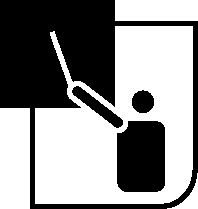
\includegraphics[width=0.75cm]{col11305.imgs/summary_presentation.png} &   \end{array} $ \hspace{2 pt}\raisebox{-5 pt}{} {(section shortcode: P10072 )} \par 
            \label{m38781*id201248}

Some materials allow electrons to move relatively freely
through them (e.g. most metals, the human body).
These materials are called \textbf{conductors}.\par 
      \label{m38781*id201271}Other materials do not allow the charge carriers, the electrons, to move
through them (e.g. plastic, glass).
The electrons are bound to the atoms in the material. These materials are called
\textbf{non-conductors} or \textbf{insulators}.\par 
      \label{m38781*id201289}If an excess of charge is placed on an insulator, it will stay
where it is put and there will be a concentration of charge in
that area of the object. However, if an excess of charge is placed
on a conductor, the like charges will repel each other
and spread out over the outside surface of the object. When two conductors
are made to touch, the total charge on them is shared between the
two. If the two conductors are identical, then each conductor will
be left with half of the total net charge.\par 
\subsection*{Arrangement of charge}
The electrostatic force determines the
arrangement of charge on the surface of conductors. This is possible because charges can move inside a conductive material. When we place
a charge on a spherical conductor the repulsive forces between the
individual like charges cause them to spread uniformly over the
surface of the sphere. However, for conductors with irregular
shapes, there is a concentration of charge near the point or points
of the object. Notice in Figure~\ref{Figure:chargedistributions} that we show a concentration of charge with more $-$ or + signs, while we represent uniformly spread charges with uniformly spaced $-$ or + signs.\par 
\Tip{The effect of the shape on the charge distribution is the reason that we only consider identical conductors for the sharing of charge.}
      \label{m38781*id201196}
    \setcounter{subfigure}{0}
	\begin{figure}[H] % horizontal\label{m38781*id201199}
    \begin{center}
\begin{pspicture}(-2,-1.2)(3.3,2)
%\psgrid
\pscircle[linewidth=1pt](-1,1){0.5}
\psline[linewidth=4pt](-1,0.5)(-1,-1)
\psline[linewidth=5pt](-1.4,-1)(-0.6,-1) \degrees[1.1]
\multido{\n=0.0+.1}{11}{%
\uput{0.6}[\n](-1,1){-}}

\psellipse[fillcolor=lightgray](2,1)(0.75,0.5)
\psline[linewidth=4pt](2,0.5)(2,-1)
\psline[linewidth=5pt](2.4,-1)(1.6,-1) \rput(3.034,1.122){-}
\rput(2.987,1.239){-} \rput(2.742,1.495){-} \rput(2.272,1.676){-}
\rput(1.728,1.676){-} \rput(1.258,1.495){-} \rput(1.013,1.239){-}
\rput(0.966,1.122){-} \rput(0.950,1.000){-} \rput(0.966,0.878){-}
\rput(1.013,0.761){-} \rput(1.258,0.505){-} \rput(1.728,0.324){-}
\rput(2.272,0.324){-} \rput(2.742,0.505){-} \rput(2.987,0.761){-}
\rput(3.034,0.878){-} \rput(3.050,1.000){-}
\end{pspicture}
    \end{center}\label{Figure:chargedistributions}
 \end{figure}       
      \IFact{This collection of charge can actually allow charge to leak off
the conductor if the point is sharp enough. It is for this reason
that buildings often have a lightning rod on the roof to remove
any charge the building has collected. This minimises the
possibility of the building being struck by lightning. This
``spreading out'' of charge would not occur if we were to place
the charge on an insulator since charge cannot move in
insulators.}

When two identical conducting spheres on insulating stands are allowed to touch they share the charge evenly between them. If the initial charge on the first sphere is ${Q}_{1}$ and the initial charge on the second sphere is ${Q}_{2}$, then the final charge on the two spheres after they have been brought into contact is:

    \begin{equation*}
    Q=\frac{{Q}_{1}+{Q}_{2}}{2}
      \end{equation*}



\section{Quantisation of charge}
            \nopagebreak
The basic unit of charge, called the elementary charge, \textsl{e}, is
the amount of charge carried by one electron.\par 

            \label{m38781*eip-97}
            \subsection{Unit of charge}
\label{m38781*eip-517}The charge on a single electron is ${q}_{e}=1,6x{10}^{-19}\phantom{\rule{2pt}{0ex}}\mathsf{C}$. All other charges in the universe consist of an integer multiple of this charge (i.e. $\mathsf{Q}={\mathsf{nq}}_{e}$). This is known as charge quantisation.      

\IFact{In 1909 Robert Millikan and Harvey Fletcher measured the charge on an electron. This experiment is now known as Millikan's oil drop experiment. Millikan and Fletcher sprayed oil droplets into the space between two charged plates and used what they knew about forces and in particular the electric force to determine the charge on an electron.}
\label{m38781*secfhsst!!!underscore!!!id290} 
      \nopagebreak
\label{m38781*id200658}Charge is measured in units called \textbf{coulombs (C)}. A coulomb of charge is a very large charge. In electrostatics we therefore often work with charge in micro-coulombs ($1\phantom{\rule{2pt}{0ex}}\mu \phantom{\rule{2pt}{0ex}}\mathsf{C}=1\ensuremath{\times}{10}^{-6}\phantom{\rule{2pt}{0ex}}\mathsf{C}$) and nanocoulombs ($1\phantom{\rule{2pt}{0ex}}\phantom{\rule{2pt}{0ex}}\mathsf{nC}=1\ensuremath{\times}{10}^{-9}\phantom{\rule{2pt}{0ex}}\mathsf{C}$).
\par 
  
\begin{wex}{Charge quantization}{An object has an excess charge of $-1,92\ensuremath{\times}{10}^{-17}\phantom{\rule{2pt}{0ex}}\mathsf{C}$. How many excess electrons does it have?}{
\westep{Analyse the problem and identify the principles}We are asked to determine a number of electrons based on a total charge. We know that charge is quantized and that electrons carry the base unit of charge which is $-1,6\ensuremath{\times}{10}^{-19}\phantom{\rule{2pt}{0ex}}\mathsf{C}$.
\westep{Apply the principle} As each electron carries the same charge the total charge must be made up of a certain number of electrons. To determine how many electrons we divide the total charge by the charge on a single electron:\label{m38781*id1166032483813}\nopagebreak\noindent{}
    \begin{eqnarray*}
N=\frac{-1,92\ensuremath{\times}{10}^{-17}}{-1,6\ensuremath{\times}{10}^{-19}}\\ 
\phantom{x}=120\phantom{\rule{2pt}{0ex}}\mathsf{electrons}
      \end{eqnarray*}}\end{wex}

\begin{wex}{Conducting spheres and movement of charge }
{I have 2 charged metal conducting spheres on insulating stands which are identical except for having different charge. Sphere A has a charge of -5 nC and sphere B has a charge of -3 nC. I then bring the spheres together so that they touch each other. Afterwards I move the two spheres apart so that they are no longer touching.\par 
      \label{m38781*id201359}\begin{enumerate}[noitemsep, label=\textbf{\arabic*}. ] 
            \leftskip=20pt\rightskip=\leftskip\label{m38781*uid7}\item What happens to the charge on the two spheres?
\label{m38781*uid8}\item What is the final charge on each sphere?
\end{enumerate}}{
      \westep{Analyse the question}\label{m38781*id201406}We have two identical negatively charged conducting spheres which are brought together to touch each other and then taken apart again. We need to explain what happens to the charge on each sphere and what the final charge on each sphere is after they are moved apart.\par 
      \westep{Identify the principles involved}
      \label{m38781*id201416}We know that the charge carriers in conductors are free to move around and that charge on a conductor spreads itself out on the surface of the conductor.\par 
      \westep{Apply the principles}
      \label{m38781*id201425}\begin{enumerate}[noitemsep, label=\textbf{\alph*}. ] 
            \leftskip=20pt\rightskip=\leftskip\label{m38781*uid9}\item When the two conducting spheres are brought together to touch, it is as though they become one single big conductor and the total charge of the two spheres spreads out across the whole surface of the touching spheres. When the spheres are moved apart again, each one is left with half of the total original charge.
\label{m38781*uid10}\item Before the spheres touch, the total charge is: -5 nC + (-3) nC = -8 nC. When they touch they share out the -8 nC across their whole surface. When they are removed from each other, each is left with half of the original charge:
\label{m38781*id201455}\nopagebreak\noindent{}
    \begin{eqnarray*}
    \frac{-8\phantom{\rule{4pt}{0ex}}\mathsf{nC}}{2}& =& -4\phantom{\rule{4pt}{0ex}}\mathsf{nC}
      \end{eqnarray*}
on each sphere.
\end{enumerate}}
\end{wex}

\begin{wex}{Identical spheres sharing charge I}{
 Two identical, insulated spheres have different charges. Sphere 1 has a charge of $-96\ensuremath{\times}{10}^{-18}~\mathsf{C}$. Sphere 2 has 60 excess electrons. If the two spheres are brought into contact and then separated, what charge will each have?}{
\westep{Analyse the question}
         We need to determine what will happen to the charge when the spheres touch. They are insulators so we know they will NOT allow charge to move freely. When they touch nothing will happen. }\end{wex}


    \begin{wex}{Identical spheres sharing charge II}{
 \label{m38781*id1166019825381}Two identical, metal spheres on insulating stands have different charges. Sphere 1 has a charge of $-9,6\ensuremath{\times}{10}^{-18}\phantom{\rule{2pt}{0ex}}\mathsf{C}$. Sphere 2 has 60 excess protons. If the two spheres are brought into contact and then separated, what charge will each have? How many electrons or protons does this correspond to?}{ We need to determine what will happen to the charge when the spheres touch. They are metal spheres so we know they will be conductors. This means that the charge is able to move so when they touch it is possible for the charge on each sphere to change. We know that charge will redistribute evenly across the two spheres because of the forces between the charges. We need to know the charge on each sphere, we have been given one.

This problem is similar to the earlier worked example. This time we have to determine the total charge given a certain number of protons. We know that charge is quantized and that protons carry the base unit of charge and are positive so it is $+1,6\ensuremath{\times}{10}^{-19}\phantom{\rule{2pt}{0ex}}\mathsf{C}$. The total charge will therefore be:\newline
$\begin{array}{ccc}{Q}_{2}=60\ensuremath{\times}1,6\ensuremath{\times}{10}^{\left(-19\right)}\phantom{\rule{2pt}{0ex}}\mathsf{C}\\ \phantom{x}=9,6\ensuremath{\times}{10}^{-18}\phantom{\rule{2pt}{0ex}}\mathsf{C}\end{array}$\par
As the spheres are identical in material, size and shape the charge will redistribute across the two spheres so that it is shared evenly. Each sphere will have half of the total charge:\newline
$\begin{array}{ccc}Q=\frac{{Q}_{1}+{Q}_{2}}{2}\\ \phantom{x}=\frac{9,6\ensuremath{\times}{10}^{-18}+\left(-9,6\ensuremath{\times}{10}^{-18}\right)}{2}\\ \phantom{x}=0\phantom{\rule{2pt}{0ex}}\mathsf{C}\end{array}$.\newline
     So each sphere is now neutral.\par
    No net charge means that there is no excess of electrons or protons.}\end{wex}
    \noindent

      \begin{wex}{Conservation of charge - 1}{Two identical, metal spheres have different charges. Sphere 1 has a charge of $-9,6\ensuremath{\times}{10}^{-18}\phantom{\rule{2pt}{0ex}}\mathsf{C}$. Sphere 2 has 30 excess electrons. If the two spheres are brought into contact and then separated, what charge will each have? How many electrons does this correspond to?}{
       \westep{Analyse the problem}
     We need to determine what will happen to the charge when the spheres touch. They are metal spheres so we know they will be conductors. This means that the charge is able to move so when they touch it is possible for the charge on each sphere to change. We know that charge will redistribute evenly across the two spheres because of the forces between the charges. We need to know the charge on each sphere, we have been given one.
\westep{Identify the principles}
     This problem is similar to the earlier worked example. This time we have to determine the total charge given a certain number of electrons. We know that charge is quantized and that electrons carry the base unit of charge which is $-1,6\ensuremath{\times}{10}^{-19}\phantom{\rule{2pt}{0ex}}\mathsf{C}$. The total charge will therefore be:
    \begin{eqnarray*}
    {Q}_{2}=30\ensuremath{\times}-1,6\ensuremath{\times}{10}^{-19}\phantom{\rule{2pt}{0ex}}\mathsf{C}\\ \phantom{x}=4,8\ensuremath{\times}{10}^{-18}\phantom{\rule{2pt}{0ex}}\mathsf{C}
      \end{eqnarray*}
    \westep{Apply the principles: redistributing charge}
     As the spheres are identical in material, size and shape the charge will redistribute across the two spheres so that it is shared evenly. Each sphere will have half of the total charge:
    \begin{eqnarray*}
Q=\frac{{Q}_{1}+{Q}_{2}}{2}\\ \phantom{x}=\frac{-9.6\ensuremath{\times}{10}^{-18}+\left(-4,8\ensuremath{\times}{10}^{-18}\right)}{2}\\ \phantom{x}=7,2\ensuremath{\times}{10}^{-18}\phantom{\rule{2pt}{0ex}}\mathsf{C}
    \end{eqnarray*}
 So each sphere now has: 
\label{m38781*id61212}\nopagebreak\noindent{}
    \begin{equation*}
    7,2\ensuremath{\times}{10}^{-18}\phantom{\rule{2pt}{0ex}}\mathsf{C}
      \end{equation*}
     of charge.\item \newline
     We know that charge is quantized and that electrons carry the base unit of charge which is $-1,6\ensuremath{\times}{10}^{-19}\phantom{\rule{2pt}{0ex}}\mathsf{C}$.
\westep{Apply the principles: charge quantisation}
     As each electron carries the same charge the total charge must be made up of a certain number of electrons. To determine how many electrons we divide the total charge by the charge on a single electron:
    \begin{eqnarray*}
     N=\frac{-7,2\ensuremath{\times}{10}^{-18}}{-1,6\ensuremath{\times}{10}^{-19}}\\ \phantom{x}=45\phantom{\rule{2pt}{0ex}}\mathsf{electrons} 
    \end{eqnarray*}
}\end{wex}




  \label{m38781*uid11}
            \begin{i_experiment}{The electroscope}
            \nopagebreak
        \label{m38781*id201715}The electroscope is a very sensitive instrument which can be used to detect electric charge.
A diagram of a gold leaf electroscope is shown the figure below. The electroscope consists of a glass container
with a metal rod inside which has 2 thin pieces of gold foil attached. The other end of the metal rod has a metal plate attached to it outside the glass container.\par 
        \label{m38781*id200543}
    \setcounter{subfigure}{0}
	\begin{figure}[H] % horizontal\label{m38781*id200546}
    \begin{center}\begin{pspicture}(0,-3.0971875)(6.2675,3.1371875)
\definecolor{color2}{rgb}{0.4,0.4,0.4}
\definecolor{color351b}{rgb}{0.6,0.6,0.6}
\psellipse[linewidth=0.04,linecolor=color2,dimen=outer](1.62,-2.6571875)(1.52,0.44)
\psline[linewidth=0.04cm,linecolor=color2](0.1,-0.0771875)(0.12,-2.6771874)
\psline[linewidth=0.04cm,linecolor=color2](3.1,-0.0771875)(3.12,-2.6771874)
\psbezier[linewidth=0.04,linecolor=color2](0.1,-0.1171875)(0.2,-0.4171875)(3.12,-0.5171875)(3.1,-0.1171875)(3.08,0.2828125)(1.74,1.2028126)(1.86,1.2428125)(1.98,1.2828125)(1.2,1.2828125)(1.36,1.2428125)(1.52,1.2028126)(0.0,0.1828125)(0.1,-0.1171875)
\psellipse[linewidth=0.04,dimen=outer,fillstyle=solid,fillcolor=color351b](1.56,1.8328125)(0.94,0.23)
\psframe[linewidth=0.04,linecolor=color2,dimen=outer,fillstyle=solid](2.5,1.9628125)(0.62,1.8228126)
\psellipse[linewidth=0.04,dimen=outer,fillstyle=solid,fillcolor=color351b](1.56,1.9328125)(0.94,0.23)
\psline[linewidth=0.04cm](0.64,1.8228126)(0.64,1.9828125)
\psline[linewidth=0.04cm](2.48,1.7828125)(2.48,1.9428124)
\psbezier[linewidth=0.04,fillstyle=solid,fillcolor=black](1.3151261,1.2328125)(1.310084,1.1228125)(1.889916,1.1355048)(1.884874,1.2328125)(1.8798319,1.3301202)(1.9,1.3258895)(1.8697479,1.3301202)(1.8394958,1.334351)(1.3907562,1.3301202)(1.3453782,1.3301202)(1.3,1.3301202)(1.320168,1.3428125)(1.3151261,1.2328125)
\psbezier[linewidth=0.04,linecolor=color2,fillstyle=solid](1.2972177,0.9730125)(1.4038053,0.9730125)(1.700252,0.9628125)(1.870126,0.9764125)(2.04,0.9900125)(2.0233457,1.3028125)(1.8601334,1.2212125)(1.6969212,1.1396126)(1.4256628,1.1728117)(1.3072103,1.2212125)(1.1887578,1.2696133)(1.1906301,0.9730125)(1.2972177,0.9730125)
\psframe[linewidth=0.04,dimen=outer,fillstyle=solid,fillcolor=black](1.66,1.6228125)(1.52,1.3428125)
\psframe[linewidth=0.04,dimen=outer,fillstyle=solid,fillcolor=black](1.68,0.9828125)(1.52,-0.0371875)
\psframe[linewidth=0.04,dimen=outer,fillstyle=solid,fillcolor=black](1.58,-0.0371875)(1.56,-0.5771875)
\psbezier[linewidth=0.04,linecolor=color2](1.5999999,-0.5534384)(1.5644444,-0.7890773)(1.4311111,-1.0328416)(1.12,-1.1384728)
\psbezier[linewidth=0.04,linecolor=color2](1.5999999,-0.5371875)(1.5644444,-0.7728263)(1.4311111,-1.0165906)(1.12,-1.1222218)
\psbezier[linewidth=0.04,linecolor=color2](1.58,-0.57343847)(1.6155556,-0.80907726)(1.748889,-1.0528415)(2.06,-1.1584728)
\psbezier[linewidth=0.04,linecolor=color2](1.58,-0.5571875)(1.6155556,-0.79282635)(1.748889,-1.0365906)(2.06,-1.1422218)
\rput{-10.598329}(-0.3782633,0.74742395){\psframe[linewidth=0.04,linecolor=color2,dimen=outer](5.54,2.6028125)(2.14,2.2228124)}
\rput(3.0746875,2.2328124){+}
\rput(2.7546875,2.3128126){+}
\rput(2.3546875,2.3928125){+}
\rput(2.0146875,2.5528126){+}
\rput(2.0546875,2.7928126){+}
\rput(2.2346876,2.9928124){+}
\rput(2.4746876,2.9528124){+}
\rput(2.7146876,2.8928125){+}
\rput(3.0546875,2.8528125){+}
\rput(3.2946875,2.7728126){+}
\rput(0.68546873,2.1528125){-}
\rput(0.98546875,2.2328124){-}
\rput(1.2454687,2.2728126){-}
\rput(1.5854688,2.2728126){-}
\rput(1.9254688,2.2528124){-}
\rput(2.1654687,2.2128124){-}
\rput(2.4254687,2.1328125){-}
\rput(2.6054688,1.9928125){-}
\rput(0.48546875,1.9928125){-}
\rput(0.46546876,1.8128124){-}
\rput(1.8146875,-0.7471875){+}
\rput(1.9546875,-0.9471875){+}
\rput(2.1946876,-1.1471875){+}
\rput(1.8746876,-1.2071875){+}
\rput(1.6746875,-1.0071875){+}
\rput(1.4946876,-1.0471874){+}
\rput(1.2746875,-1.2271875){+}
\rput(1.0146875,-1.0671875){+}
\rput(1.2546875,-0.9271875){+}
\rput(1.3946875,-0.7471875){+}
\psline[linewidth=0.027999999cm,linecolor=color2](1.68,-0.7771875)(4.02,-0.7771875)
\psline[linewidth=0.04cm,linecolor=color2](2.22,1.9828125)(4.0,1.1628125)
\psline[linewidth=0.04cm,linecolor=color2](3.86,2.2428124)(4.12,1.7628125)
\rput(5.1584377,-0.7471875){gold foil leaves}
\rput(4.8932815,1.1128125){metal plate}
\rput(5.044375,1.6728125){charged rod}
\psline[linewidth=0.04cm,linecolor=color2](3.1,-2.1771874)(4.0,-2.1771874)
\rput(5.065781,-2.1471875){glass container}
\end{pspicture}
    \end{center}
 \end{figure}       
        \par 
        \label{m38781*id200552}The electroscope detects charge in the following way: A charged object, like the positively charged rod in the picture, is brought close to (but not touching) the neutral metal plate of the electroscope. This causes negative charge in the gold foil, metal rod, and metal plate, to be attracted to the positive rod. Because the metal (gold is a metal too!) is a conductor, the charge can move freely from the foil up the metal rod and onto the metal plate. There is now more negative charge on the plate and more positive charge on the gold foil leaves. This is called \textsl{inducing} a charge on the metal plate. It is important to remember that the electroscope is still neutral (the total positive and negative charges are the same), the charges have just been induced to \textsl{move} to different parts of the instrument! The induced positive charge on the gold leaves forces them apart since like charges repel! This is how we can tell that the rod is charged. If the rod is now moved away from the metal plate, the charge in the electroscope will spread itself out evenly again and the leaves will fall down because there will no longer be an induced charge on them.\par 
        \label{m38781*uid12}

            \subsubsection{Grounding}
            \nopagebreak
          \label{m38781*id200585}If you were to bring the charged rod close to the uncharged electroscope, and then you touched the metal plate with your finger at the same time, this would cause charge to flow up from the ground (the earth), through your body onto the metal plate. Connecting to the earth so charge flows is called \textbf{grounding}. The charge flowing onto the plate is opposite to the charge on the rod, since it is attracted to the charge on the rod. Therefore, for our picture, the charge flowing onto the plate would be negative. Now that charge has been added to the electroscope, it is no longer neutral, but has an excess of negative charge. Now if we move the rod away, the leaves will remain apart because they have an excess of negative charge and they repel each other. If we ground the electroscope again (this time without the charged rod nearby), the excess charge will flow back into the earth, leaving it neutral.\par 
          \label{m38781*id200601}
    \setcounter{subfigure}{0}
	\begin{figure}[H] % horizontal\label{m38781*id200605}
    \begin{center}
%     \scalebox{0.8} % Change this value to rescale the drawing.
% {
\begin{pspicture}(0,-2.7271874)(7.7496877,2.7671876)
\definecolor{color2}{rgb}{0.4,0.4,0.4}
\definecolor{color351b}{rgb}{0.6,0.6,0.6}
\psellipse[linewidth=0.04,linecolor=color2,dimen=outer](1.62,-2.2871876)(1.52,0.44)
\psline[linewidth=0.04cm,linecolor=color2](0.1,0.2928125)(0.12,-2.3071876)
\psline[linewidth=0.04cm,linecolor=color2](3.1,0.2928125)(3.12,-2.3071876)
\psbezier[linewidth=0.04,linecolor=color2](0.1,0.2528125)(0.2,-0.0471875)(3.12,-0.1471875)(3.1,0.2528125)(3.08,0.6528125)(1.74,1.5728126)(1.86,1.6128125)(1.98,1.6528125)(1.2,1.6528125)(1.36,1.6128125)(1.52,1.5728126)(0.0,0.5528125)(0.1,0.2528125)
\psellipse[linewidth=0.04,dimen=outer,fillstyle=solid,fillcolor=color351b](1.56,2.2028124)(0.94,0.23)
\psframe[linewidth=0.04,linecolor=color2,dimen=outer,fillstyle=solid](2.5,2.3328125)(0.62,2.1928124)
\psellipse[linewidth=0.04,dimen=outer,fillstyle=solid,fillcolor=color351b](1.56,2.3028126)(0.94,0.23)
\psline[linewidth=0.04cm](0.64,2.1928124)(0.64,2.3528125)
\psline[linewidth=0.04cm](2.48,2.1528125)(2.48,2.3128126)
\psbezier[linewidth=0.04,fillstyle=solid,fillcolor=black](1.3151261,1.6028125)(1.310084,1.4928125)(1.889916,1.5055048)(1.884874,1.6028125)(1.8798319,1.7001202)(1.9,1.6958895)(1.8697479,1.7001202)(1.8394958,1.704351)(1.3907562,1.7001202)(1.3453782,1.7001202)(1.3,1.7001202)(1.320168,1.7128125)(1.3151261,1.6028125)
\psbezier[linewidth=0.04,linecolor=color2,fillstyle=solid](1.2972177,1.3430125)(1.4038053,1.3430125)(1.700252,1.3328125)(1.870126,1.3464125)(2.04,1.3600125)(2.0233457,1.6728125)(1.8601334,1.5912125)(1.6969212,1.5096124)(1.4256628,1.5428118)(1.3072103,1.5912125)(1.1887578,1.6396133)(1.1906301,1.3430125)(1.2972177,1.3430125)
\psframe[linewidth=0.04,dimen=outer,fillstyle=solid,fillcolor=black](1.66,1.9928125)(1.52,1.7128125)
\psframe[linewidth=0.04,dimen=outer,fillstyle=solid,fillcolor=black](1.68,1.3528125)(1.52,0.3328125)
\psframe[linewidth=0.04,dimen=outer,fillstyle=solid,fillcolor=black](1.58,0.3328125)(1.56,-0.2071875)
\psbezier[linewidth=0.04,linecolor=color2](1.5999999,-0.18343845)(1.5644444,-0.41907728)(1.4311111,-0.66284156)(1.12,-0.7684728)
\psbezier[linewidth=0.04,linecolor=color2](1.5999999,-0.1671875)(1.5644444,-0.40282634)(1.4311111,-0.64659065)(1.12,-0.7522218)
\psbezier[linewidth=0.04,linecolor=color2](1.58,-0.20343846)(1.6155556,-0.4390773)(1.748889,-0.6828416)(2.06,-0.7884728)
\psbezier[linewidth=0.04,linecolor=color2](1.58,-0.1871875)(1.6155556,-0.42282632)(1.748889,-0.66659063)(2.06,-0.7722218)
\rput(0.68546873,2.5228126){-}
\rput(0.98546875,2.6028125){-}
\rput(1.4054687,0.7028125){-}
\rput(1.5854688,2.6428125){-}
\rput(1.8254688,0.8428125){-}
\rput(1.3054688,-0.7771875){-}
\rput(2.4254687,2.5028124){-}
\rput(2.6054688,2.3628125){-}
\rput(0.48546875,2.3628125){-}
\rput(1.8346875,2.6028125){+}
\rput(1.9546875,-0.5771875){+}
\rput(1.7346874,-0.3171875){+}
\rput(1.8546875,1.0228125){+}
\rput(2.2346876,2.5428126){+}
\rput(1.3146875,-0.4371875){+}
\rput(1.8346875,0.3228125){+}
\rput(0.8146875,2.5628126){+}
\rput(1.3146875,2.6228125){+}
\rput(1.4146875,0.3428125){+}
\psline[linewidth=0.027999999cm,linecolor=color2](1.68,-0.4071875)(4.02,-0.4071875)
\psline[linewidth=0.04cm,linecolor=color2](2.22,2.3528125)(4.0,1.5328125)
\rput(5.523594,-0.3771875){gold foil leaves with}
\rput(4.8932815,1.4828125){metal plate}
\psline[linewidth=0.04cm,linecolor=color2](3.1,-1.8071876)(4.0,-1.8071876)
\rput(5.065781,-1.7771875){glass container}
\rput(0.46546876,2.1828125){-}
\rput(2.0254688,2.6228125){-}
\rput(1.8454688,0.5628125){-}
\rput(1.4254688,0.1428125){-}
\rput(1.3854687,-0.2571875){-}
\rput(1.8454688,-0.4771875){-}
\rput(2.1454687,-0.7371875){-}
\rput(1.7454687,-0.6971875){-}
\rput(1.6254687,-0.5171875){-}
\rput(1.4654688,-0.6371875){-}
\rput(1.2254688,-0.5771875){-}
\rput(0.96546876,-0.6771875){-}
\rput(1.7654687,0.1228125){-}
\rput(1.4254688,0.9628125){-}
\rput(1.4254688,1.1628125){-}
\rput(1.8654687,-0.7771875){-}
\rput(5.888125,-0.7371875){excess of negative charge}
\rput(5.25,-1.0571876){repel each other}
\rput(1.1854688,2.6228125){-}
\rput(2.5054688,2.0628126){-}
\end{pspicture}
%}
\end{center}
 \end{figure}       
\end{i_experiment}
            
            \section{Summary}
            \nopagebreak
      \label{m38781*id201947}\begin{enumerate}[noitemsep, label=\textbf{\arabic*}. ] 
\item There are two kinds of charge.
            \label{m38781*uid14}\item Objects can be \textbf{positively} charged, \textbf{negatively} charged or \textbf{neutral}.
\label{m38781*uid15}\item Objects that are neutral have equal numbers of positive and negative charge.

\label{m38781*uid16}\item Unlike charges are attracted to each other and like charges are repelled from each other.
\label{m38781*uid17}\item Charge is neither created nor destroyed, it can only be transferred.
\label{m38781*uid18}\item Charge is measured in coulombs (C).
\item Charge is quantised in units of the charge of an electron $1.6\times10^{-19}~\mathsf{C}$.
\label{m38781*uid19}\item Conductors allow charge to move through them easily.
\label{m38781*uid20}\item Insulators do not allow charge to move through them easily.
\item Identical, conducting sphere in contact share their charge according to:
\begin{equation*}
 Q=\frac{Q_1+Q_2}{2}
\end{equation*}
\end{enumerate}
        \label{m38781*eip-152}The following presentation is a summary of the work covered in this chapter. Note that the last two slides are not needed for exam purposes, but are included for general interest.\newline
    \setcounter{subfigure}{0}
	\begin{figure}[H] % horizontal\label{m38781*slidesharefigure}
    \label{m38781*slidesharemedia}\label{m38781*slideshareflash}\raisebox{-5 pt}{ 
\includegraphics[width=0.5cm]{col11305.imgs/summary_www.png}} { (Presentation:  P10073 )}
 \end{figure}       \par 
    \label{m38781*cid10}
            \begin{eocexercises}{Electrostatics}
            \nopagebreak
      \label{m38781*id202059}\begin{enumerate}[noitemsep, label=\textbf{\arabic*}. ] 
            \label{m38781*uid21}\item What are the two types of charge called?\newline
\label{m38781*uid22}\item Provide evidence for the existence of two types of charge.\newline
\label{m38781*uid23}\item Fill in the blanks: The electrostatic force between like charges is  \uline{\hspace{10ex}}
 while the electrostatic force between opposite charges is  \uline{\hspace{10ex}}
.\newline
\label{m38781*uid24}\item I have two positively charged metal balls placed 2 m apart.
\label{m38781*id202122}\begin{enumerate}[noitemsep, label=\textbf{\alph*}. ] 
            \label{m38781*uid25}\item Is the electrostatic force between the balls attractive or repulsive?
\label{m38781*uid26}\item If I now move the balls so that they are 1 m apart, what happens to the strength of the electrostatic force between them?
\end{enumerate}
        \newline
            \label{m38781*uid27}\item I have 2 charged spheres each hanging from string as shown in the picture below.
    \setcounter{subfigure}{0}
	\begin{figure}[H] % horizontal\label{m38781*id202166}
    \begin{center}
    \begin{pspicture}(0,-1.23)(2.74,1.25)
\pscircle[linewidth=0.04,dimen=outer](0.41,-0.82){0.41}
\pscircle[linewidth=0.04,dimen=outer](2.33,-0.82){0.41}
\psline[linewidth=0.04cm](0.4,-0.43)(0.4,1.23)
\psline[linewidth=0.04cm](2.34,-0.45)(2.34,1.21)
\rput(2.3559375,-0.815){\large +}
\rput(0.3790625,-0.835){\large +}
\end{pspicture}\end{center}
 \end{figure}       
Choose the correct answer from the options below:
The spheres will
\label{m38781*id202176}\begin{enumerate}[noitemsep, label=\textbf{\alph*}. ] 
            \label{m38781*uid28}\item swing towards each other due to the attractive electrostatic force between them.
\label{m38781*uid29}\item swing away from each other due to the attractive electrostatic force between them.
\label{m38781*uid30}\item swing towards each other due to the repulsive electrostatic force between them.
\label{m38781*uid31}\item swing away from each other due to the repulsive electrostatic force between them.
\end{enumerate}
        \newline
            \label{m38781*uid32}\item Describe how objects (insulators) can be charged by contact or rubbing.\newline
\label{m38781*uid33}\item You are given a perspex ruler and a piece of cloth.
\label{m38781*id202255}\begin{enumerate}[noitemsep, label=\textbf{\alph*}. ] 
            \label{m38781*uid34}\item How would you charge the perspex ruler?
\label{m38781*uid35}\item Explain how the ruler becomes charged in terms of charge.
\label{m38781*uid36}\item How does the charged ruler attract small pieces of paper?
\end{enumerate}
        \newline
            \label{m38781*uid37}\item (IEB 2005/11 HG) An uncharged hollow metal sphere is placed on an insulating stand. A positively charged rod is brought up to touch the hollow metal sphere at P as shown in the diagram below. It is then moved away from the sphere.
    \setcounter{subfigure}{0}
	\begin{figure}[H] % horizontal\label{m38781*id202314}
    \begin{center}
    \begin{pspicture}(-1,0)(1,3.2)
\SpecialCoor
%\psgrid[gridcolor=lightgray]
\psframe(-1,0)(1,0.2) \psframe(-0.1,0.2)(0.1,2.2)
\pscircle[fillcolor=white,fillstyle=solid](0,2.7){0.5}
\psellipse[fillcolor=white,fillstyle=solid](0.4,3)(0.1,0.2)
\psframe[fillcolor=white,fillstyle=solid,linestyle=none](0.4,2.8)(2.4,3.2)
\psline(0.4,2.8)(2.4,2.8) \psline(0.4,3.2)(2.4,3.2)
\rput(2,0){\psellipse[fillcolor=white,fillstyle=solid](0.4,3)(0.1,0.2)}
\uput[dl](0.4,3){P} \uput[r](0.4,3){+++}
\end{pspicture}\end{center}
 \end{figure}       
Where is the excess charge distributed on the sphere after the rod
has been removed?
\label{m38781*id202325}\begin{enumerate}[noitemsep, label=\textbf{\alph*}. ] 
            \label{m38781*uid38}\item It is still located at point P where the rod touched the sphere.
\label{m38781*uid39}\item It is evenly distributed over the outer surface of the hollow sphere.
\label{m38781*uid40}\item It is evenly distributed over the outer and inner surfaces of the hollow sphere.
\label{m38781*uid41}\item No charge remains on the hollow sphere.
\end{enumerate}
        \newline
            \label{m38781*uid42}\item What is the process called where molecules in an uncharged object are caused to align in a particular direction due to an external charge?\newline
\label{m38781*uid43}\item Explain how an uncharged object can be attracted to a charged object. You should use diagrams to illustrate your answer.\newline
\label{m38781*uid44}\item Explain how a stream of water can be attracted to a charged rod.\newline
\item An object has an excess charge of 
$-8,6\ensuremath{\times}{10}^{-18}\phantom{\rule{2pt}{0ex}}\mathsf{C}$. How many excess electrons does it have?\newline
            \item An object has an excess of 235 electrons. What is the charge on the object?\newline
            \item An object has an excess of 235 protons. What is the charge on the object?\newline
            \item Two identical, metal spheres have different charges. Sphere 1 has a charge of 
$-4,8\ensuremath{\times}{10}^{-18}\phantom{\rule{2pt}{0ex}}\mathsf{C}$. Sphere 2 has 60 excess electrons. If the two spheres are brought into contact and then separated, what charge will each have? How many electrons does this correspond to?\newline
            \item Two identical, insulated spheres have different charges. Sphere 1 has a charge of 
$-96\ensuremath{\times}{10}^{-18}\phantom{\rule{2pt}{0ex}}C$. Sphere 2 has 60 excess electrons. If the two spheres are brought into contact and then separated, what charge will each have? \newline
            \item Two identical, metal spheres have different charges. Sphere 1 has a charge of 
$-4,8\ensuremath{\times}{10}^{-18}\phantom{\rule{2pt}{0ex}}\mathsf{C}$. Sphere 2 has 30 excess protons. If the two spheres are brought into contact and then separated, what charge will each have? How many electrons or protons does this correspond to?\newline
            \end{enumerate}
  \label{m38781**end}
  \label{464e844ca5615087ea89d9d95dd9a43a**end}
\par \raisebox{-5 pt}{
\includegraphics[width=0.5cm]{col11305.imgs/summary_www.png}} Find the answers with the shortcodes:
 \par \begin{tabular}[h]{cccccc}
 (1.) lqs  &  (2.) lqo  &  (3.) lqA  &  (4.) lqG  &  (5.) lqf  &  (6.) lqw  &  (7.) lqv  &  (8.) lqd  &  (9.) ljH  &  (10.) la2  &  (11.) lqP  &  (12.) lTf  &  (13.) lTG  &  (14.) lT7  &  (15.) lTA  &  (16.) lTo  &  (17.) lTs  & \end{tabular}
\end{eocexercises}